\section{Resultados}
%Deben incluir los resultados de los experimentos, utilizando el formato más adecuado
%para su presentación. Deberón especificar claramente a qué experiencia corresponde
%cada resultado. No se incluirán aquí corridas de máquina. Algo fundamental en su
%aprendizaje en la materia es la presentación de resultados de forma clara y concisa para
%el lector.
\subsection{Experimento relación tiempo-calidad de cómputo}
Las siguientes tres tablas representan los datos tomados de tres instancias del problema. Lo único que vamos a variar en dichas instancias son los radios de las sanguijuelas. Para las tres instancias $a = 20$, $b = 20$, la cantidad de sanguijuelas es 8 y las ubicaciones y temperaturas (variando en un rango de 50 a 730) de cada sanguijuela son las mismas (pueden encontrarse en los archivos de Experimentos/Experimento2/instancias20x20).
\newline
\begin{figure}[H]
\centering
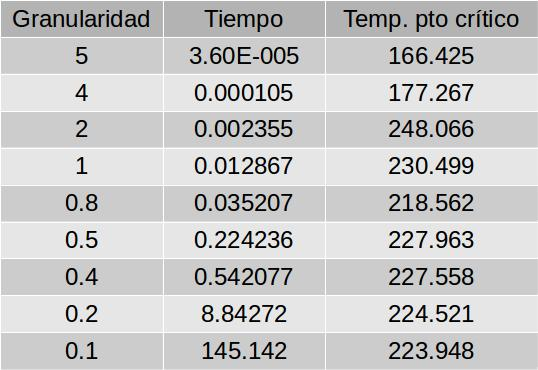
\includegraphics[scale=0.4]{../../Experimentos/Experimento2/instancia20x20_1.jpg}\caption{En este conjunto de instancias los radios de las sanguijuelas están en el conjunto $\{2, 3, 4\}$. Podemos observar como efectivamente el tiempo crece cuando el parámetro $h$ de granularidad disminuye. En cuanto a la temperatura del punto crítico, se puede ver como a medida que aumentamos el tamaño de nuestras discretizaciones, se va acercando a un valor cercano a 224 grados.}
\end{figure}

\begin{figure}[H]
\centering
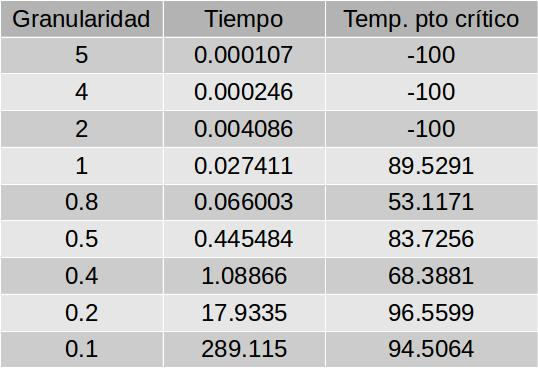
\includegraphics[scale=0.4]{../../Experimentos/Experimento2/instancia20x20_2.jpg}\caption{En este otro experimento, hemos decidido achicar considerablemente los radios de las sanguijuelas de manera que estén en el rango $[0.03, 1]$. Por un lado, podemos ver que el tiempo sigue aumentando a medida que $h$ disminuye al igual que en el experimento anterior. Sin embargo, se puede ver también que el algoritmo toma más tiempo que antes en resolver cada instancia. De todas formas, lo más llamativo parece encontrarse en las primeras tres entradas de la tabla, en los valores de temperatura del punto crítico. Pareciera como si las primeras tres discretizaciones de nuestro modelo del problema, aproximan tan mal al caso real que quedan descartadas todas las sanguijuelas. Sin embargo, al igual que en el experimento anterior, se cumple que a medida que aumenta el tamaño de la discretización, la temperatura en el punto crítico se acerca a un valor.}
\end{figure}

\begin{figure}[H]
\centering
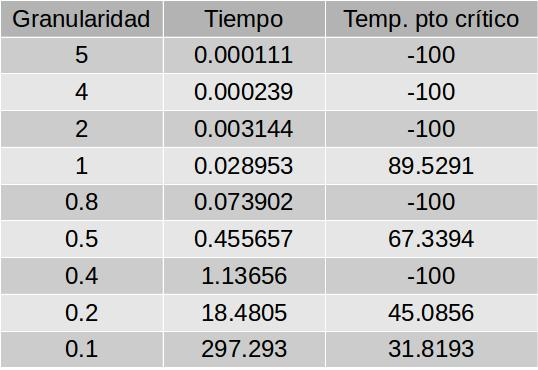
\includegraphics[scale=0.4]{../../Experimentos/Experimento2/instancia20x20_3.jpg}\caption{Una vez más, volvemos a achicar los radios de las sanguijuelas. Vemos que el tiempo se sigue comportando de manera similar y con las primeras tres instancias del problema ocurre lo mismo que con el experimento anterior. Sin embargo, ahora si está sucediendo algo que contradice una de las hipótesis (la tercera) planteada en el desarrollo ya que vemos que ahora, no pareciera que nos estemos acercando a un valor (el valor de la solución real). Esto se ve en las entradas 6 y 7 de la tabla, cuyas granularidades son 0.8 y 0.4, donde a pesar de que son más chicas que 1 (y por lo tanto las discretizaciones poseen tamaños más grandes), se está obteniendo -100 como temperatura del punto crítico, lo cuál no parece estar bien.}
\end{figure}

\begin{figure}[H]
\centering
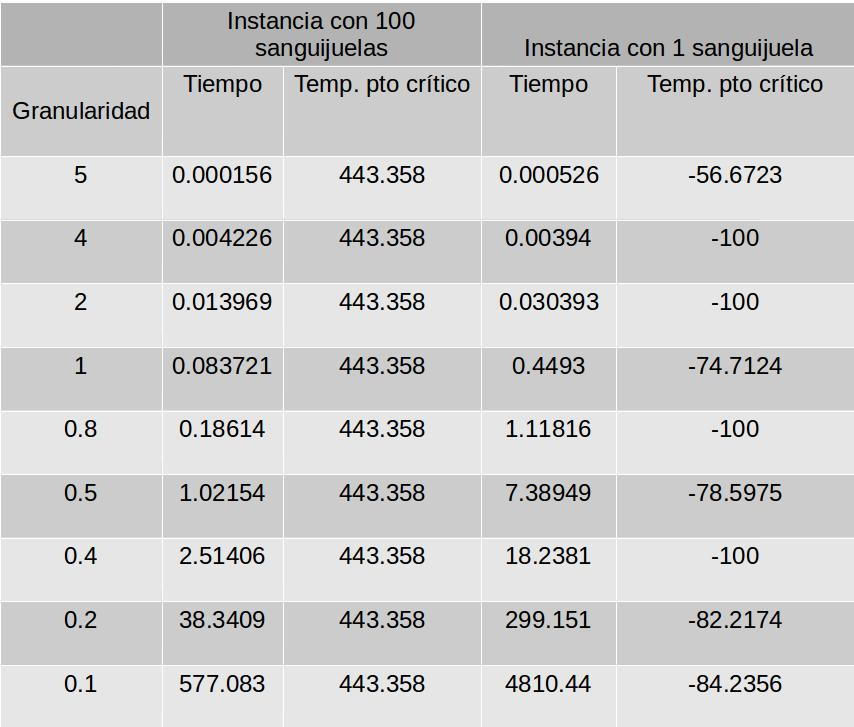
\includegraphics[scale=0.4]{../../Experimentos/Experimento2/instancias40x40.jpg}\caption{En este experimento se trabajó con dos instancias, esta vez ambas de 40x40 y con distintas sanguijuelas asociadas a una y a otra. Más específicamente y como indica la tabla, en una instancia hay 100 sanguijuelas y en la otra solo 1. Los radios de las 100 sanguijuelas se generaron con distribución uniforme en el rango [25, 35] mientras que radio de la única sanguijuela de la segunda instancia es de 0.002.  Vemos como estos resultados entran en conflicto con la hipótesis 2 ya que los tiempos medidos de la instancia con 1 sanguijuela son mucho más largos que con la instancia de 100 sanguijuelas. También podemos observar algo interesante acerca de la instancia con 100 sanguijuelas y esto es que, la temperatura en el punto crítico siempre fue la misma. }
\end{figure}

\begin{figure}[H]
\centering
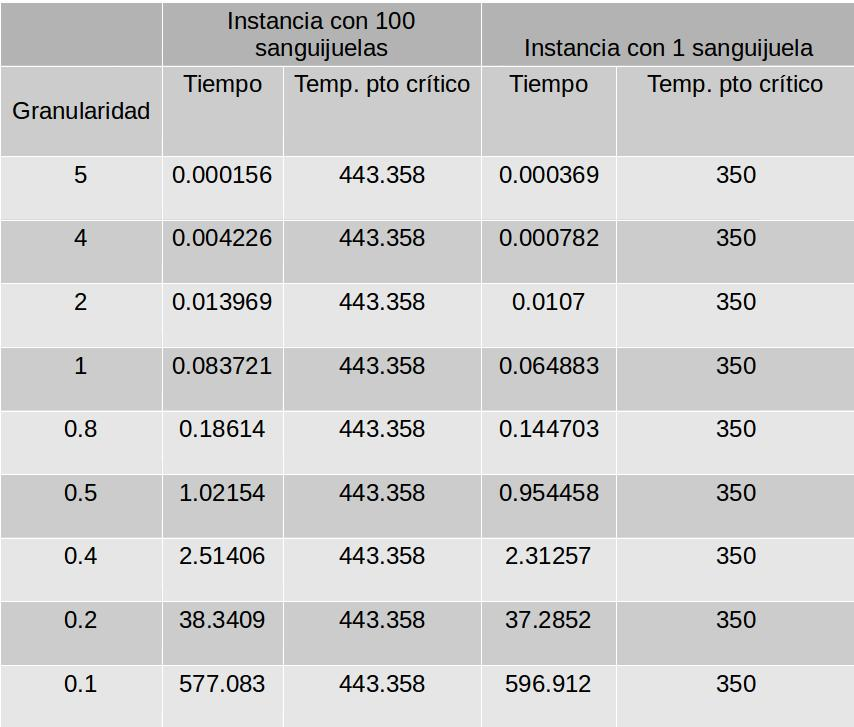
\includegraphics[scale=0.4]{../../Experimentos/Experimento2/instancias40x40_2.jpg}\caption{Para hacer esta última medición, decidimos dejar intacta la instancia con 100 sanguijuelas y modificar la instancia que tiene solo una sanguijuela. La modificación que efectuamos fue aumentar considerablemente el radio de la sanguijuela a un valor de 40, siendo antes 0.002. Podemos observar que los tiempos son significativamente menores, parecidos a los que tomamos al trabajar con la instancia de 100 sanguijuelas e incluso en algunos casos menores. Es importante observar también, que la temperatura en el punto crítico ahora es siempre la misma (350) y antes (cuando el radio era 0.002) variaba y a veces la sanguijuela era descartada (para las granularidades 4, 2, 0.8 y 0.4 de la tabla anterior).}
\end{figure}